\section{Accessibilità}

\subsection{Separazione tra contenuto, presentazione e struttura}
Per migliorare l'accesso al sito agli utenti con differenti disabilità e ai motori di ricerca è stata mantenuta la separazione tra struttura, presentazione e comportamento. 
La prima è stata sviluppata tramite documenti XHTML Strict 1.0 e HTML5, i quali richiamano i fogli di stile esterni CSS che implementano la presentazione e script esterni realizzati con JavaScript che formano il comportamento. Questi script sono stati implementati in modo da garantire una trasformazione elegante del sito, poiché se JavaScript è disabilitato il contenuto rimane comunque accessibile; maggiori informazioni riguardo il comportamento del sito si possono trovare alla sezione \ref{js}.\\ 
Tutto il codice redatto è stato scritto secondo le raccomandazioni W3C, accertando che fossero state rispettate tramite validazione (Sezione \ref{valid}). Si è evitato l'uso di tag e attributi deprecati.\\

\subsection{Schema colori}
Si è cercato di utilizzare uno schema colori tale che garantisca un contrasto elevato, in modo da facilitare la lettura del contenuto anche alle persone con disturbi visivi come il daltonismo.\\
Inoltre, per evitare di confondere le persone con problemi visivi, i link vengono sempre rappresentati sottolineati e sempre dello stesso colore, fatta eccezione per le barre di navigazione dove è comunque chiaro che le voci che compaiono sono link.

Per garantire che il sito sia accessibile anche alle persone con disturbi visivi è stato utilizzato il servizio offerto dal sito  \url{http://www.vischeck.com/} che a partire da uno screenshot di una pagina, mostra come viene visualizzata da persone con determinati disturbi visivi. Viene di seguito riportato il risultato ottenuto dal test della home page.

\begin{figure}
\centering
\begin{subfigure}{.5\textwidth}
  \centering
  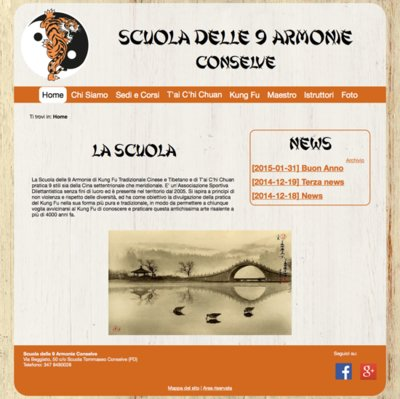
\includegraphics[width=.9\linewidth]{../immagini/originale.jpg}
  \caption{Pagina originale}
  \label{fig:sub1}
\end{subfigure}%
\begin{subfigure}{.5\textwidth}
  \centering
  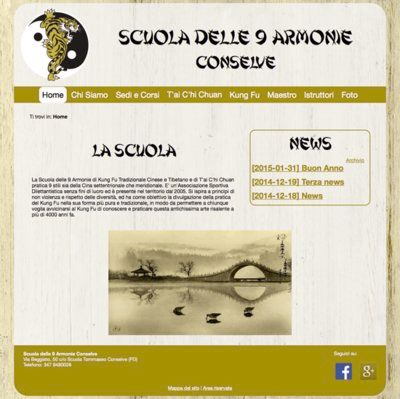
\includegraphics[width=.9\linewidth]{../immagini/deutranope.jpg}
  \caption{Pagina vista da un deutranope}
  \label{fig:sub2}
\end{subfigure}
\begin{subfigure}{.5\textwidth}
  \centering
  
\includegraphics[width=.9\linewidth]{../immagini/protranope.jpg}
  \caption{Pagina vista da un protranope}
  \label{fig:sub3}
\end{subfigure}%
\begin{subfigure}{.5\textwidth}
  \centering
  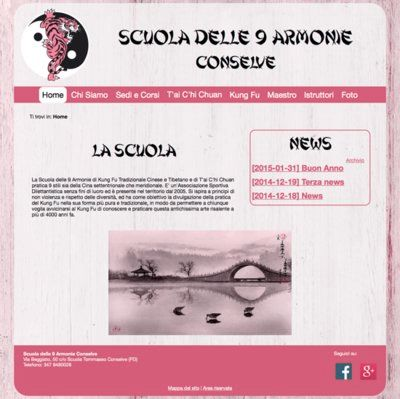
\includegraphics[width=.9\linewidth]{../immagini/tritranope.jpg}
  \caption{Pagina vista da un tritranope}
  \label{fig:sub4}
\end{subfigure}

\caption{Homepage vista da persone con problemi nel distinguere i colori}
\label{fig:test}
\end{figure}

\FloatBarrier


\subsection{Tag meta}
Sono stati inseriti per ogni pagina i tag meta: \texttt{Content-Type}, \texttt{keywords}, \texttt{description}, \texttt{author} e \texttt{languages} e il tag \texttt{title}, il quale descrive la pagina corrente dal particolare al generale. \\
Il tag \texttt{languages} indica che il sito è stato interamente scritto in italiano ma compaiono alcune parole inglesi, le quali sono state affiancate dall'attributo: \texttt{xml:lang=''en''}.\\
Essendo il sito dedicato ad un arte marziale cinese compaiono inevitabilmente alcuni vocaboli orientali, scritti comunque in latino, i quali sono stati segnalati agli screen reader tramite uno \texttt{<span title=''...''></span>}, dove all'interno dell'attributo title è stata riportata la pronucia del vocabolo cinese. 


\subsection{Screen reader}

Ogni foto di contenuto è stata arricchita di attributi \texttt{alt} e \texttt{title} che descrivono in maniera esaustiva ciò che l'immagine ritrae. Per le immagini che sono state ritenute non di contenuto, e che sono così state inserite tramite CSS, non è stato previsto l'uso di questi attributi, ritenendo la loro unica funzione quella di abbellimento, non portando informazione utile per la comprensione della pagina.

Mai sono state utilizzate immagni per riportare il testo, perciò il contenuto informativo rimane accessibile anche quando fallisce il caricamento delle immagini o del CSS.

Ogni campo di un \texttt{form} è stato sempre corredato con una etichetta \texttt{label} e le varie voci sono state sempre raggruppate in \texttt{fieldset}.

\subsection{Facilitazioni per la navigazione}

Al fine di agevolare la visita al sito da parte degli utenti con disabilità si sono predisposte le seguenti facilitazioni:
\begin{itemize}
\item \textbf{Tabindex:} Per ogni pagina sono stati ridefiniti i \texttt{tabindex}. Ad ogni pressione del tasto tab il focus si sposta sul link direttamente successivo per agevolare la navigazione, specialmente nella navbar;
\item \textbf{Link per spostarsi al contenuto:} Prima della navbar è stato inserito un link, nascosto all'utenza normale, ma che permette agli utenti che visualizzano il sito mediante uno screen reader di saltare la barra di navigazione;
\item \textbf{Link per tornare al menù:} Per facilitare la visita del sito, sia agli utenti che utilizzano screen reader, sia agli utenti che visualizzano il sito in versione mobile, sono stati predisposti dei link, alla fine dei paragrafi che permettono di tornare alla barra di navigazione.
\end{itemize}


\section{Usabilità}

Particolare attenzione è stata posta all'usabilità del sito e si è cercato dunque di rispettare il più possibile le sue raccomandazioni:
\begin{itemize}
\item \textbf{Le sei W:} La home page del sito risponde alle seguenti domande: 

\begin{itemize}

\item \textit{Where:}
Il breve testo presente nelle pagina di apertura illustra in maniera esaustiva ciò che il sito si propone di rappresentare, ovvero la Scuola delle 9 Armonie Conselve, dove si praticano arti marziali cinesi e tibetane;

\item \textit{Who:}
Un utente che accede per la prima volta ad un sito sente la necessità di conoscere chi o quale entità il esso rappresenta. Abbiamo 	quindi posizionato, come di consueto, in alto a sinistra il logo della scuola e subito affianco il nome. Il logo è cliccabile in ogni pagina e riporta sempre alla home page; 

\item \textit{When:}
Nella sezione news vengono riportate le ultime comunicazioni che la scuola manda ai propri allievi, soprattutto per quanto riguarda attività extra ordinarie e stage nel fine settimana. A queste comunicazioni sono associate le relative date, in modo da dare all'utente l'idea di quando è stato aggiornato l'ultima volta il sito;

\item \textit{How:}
La barra di navigazione illustra tutte le sezioni principali del sito alle quali un utente non autenticato può accedere;

\item \textit{What:}
Un utente, quando accede alla home page riesce a farsi un'idea delle offerte del sito, infatti, grazie al titolo \textit{La Scuola} e alle varie sezioni della navbar: \textit{Sedi e Corsi}, \textit{Kung Fu} e \textit{T'ai C'hi Chuan} è facilmente intuibile che il sito offra delle informazioni riguardo ad una scuola di arti marziali.

\end{itemize}

\item \textbf{Navbar:} Viene sempre evidenziata la voce della pagina in cui siamo all'interno della barra di navigazione. Essa non è cliccabile, evitando così un refresh inutile. Anche quando è puntata dal mouse una voce viene evidenziata, suggerendo all'utente che essa è un link e porta così ad un altra sezione.

\item \textbf{Breadcrumbs:} Affinché l'utente non si perda mai all'interno del sito, è stato riportato, sotto la barra di navigazione, il percorso che si è effettuato dall'home page. Anche se l'annidamento è esiguo e al massimo si è raggiunto il terzo livello, nella sezione dei singoli istruttori, si è pensato ad una futura, e molto probabile, espansione del sito.

\item \textbf{Link:} Ogni link è di un colore differente rispetto ad una semplice parola del testo ed è stato sottolineato. Non presenta la classica colorazione viola perché si è scelto un colore che richiami le tonalità principali del sito. Ogni link che è già stato visitato riporta un colore più scuro rispetto all'originale, suggerendo così all'utente le pagine che ha già visualizzato.

\item \textbf{Foto:} Ogni immagine è nitida e ben visibile. Per ogni foto di contenuto si è pensato ad una sua espansione tramite una libreria che verrà illustrata nella sezione \ref{js}. Purtroppo lo spazio a disposizione nel server Universitario non permette il caricamento di foto dettagliate e di grandi dimensioni. Perciò si è limitata questa possibilità alla sola galleria fotografica.  
\end{itemize}
